\documentclass{article}
\usepackage{amssymb}
\usepackage{amsmath}
\usepackage{fancyhdr}
\usepackage{booktabs}
\usepackage{harvard}
\usepackage[hidelinks]{hyperref}
\citationmode{abbr}
\citationstyle{dcu}
\pagestyle{fancy}
\usepackage{graphicx}
\graphicspath{ {images/} }
\lhead{Justin Coker | Problem Set 7}
\rhead{}
\begin{document}
\section{Data and Description}

The data used for this exercise is provided by Eurostat, the statistical office of the European Union. The data can be found at http://ec.europa.eu/eurostat/da
ta/database. In particular, I am using Per Capita R&D expenditure data at the Nomenclature of Territorial Units for Statistics (NUTS 2) level. This data was accessed in json format using the pyjstat module to access a customized url generated using Eurostat's query builder.\\

My plan in using this data is to identify spatial spillover of innovation activity across national borders. I hope to use a neighbor country's joining of the EU as a shock to innovation spillover across borders (the assumption being that cross-border travel should be easier ex-post). Using the neighbors.py (credit: Ujaval Gandhi, http://www.qgistutorials.com/en/docs/find\_neighbor\_polygons.html) I can identify NUTS 2 regions that lie along the border of any country which joined the EU in 2004 (``Border Regions"). Similarly, I can identify NUTS 2 regions that do not lie along such a border (``Interior Regions").

The 2004 joining countries are: Czech Republic, Estonia, Hungary, Latvia, Lithuania, Malta, Poland, Slovakia, Slovenia.\\

My goal is to use interior regions as the control group and border regions as the treatment group, the treatment being the fact that a neighbor country has joined the EU.\\

Causal Inference in this case requires that we control for economic factors that affect R&D activity in all regions (interior or otherwise) such as Recessions, Political Institutions, etc. I posit, therefore, that a difference in difference (``DiD") strategy may be best suited to this situation.\\

Before performing any econometric analysis, it is important to check the visual evidence for validity of the DiD strategy. The graph below shows average R&D expenditure for interior regions (Red line) and border regions (Blue line). 

Unfortunately, at least at the aggregate levels, it appears that causal inference using a DiD will be impossible. First, the parallel pre-trend assumption appears to be violated. It seems that prior to 2004, R&D activity in border regions was declining at least until 2001 while interior regions saw stable growth over this period.

In addition, post 2004, we seem to have parallel trends for border and interior regions. Visually, it appears that a DiD estimation would not pick up any spillover effect in this case. Additionally, any effect identified by the DiD would be biased given the failure of the pre-trend assumption.
\newpage
\section*{Figure 1}
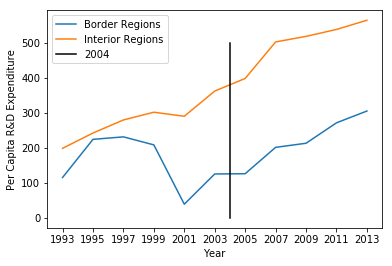
\includegraphics[scale = .65]{Plot}






\end{document}